\documentclass[tikz,border=5mm]{standalone}
\usepackage{tikz}
\usetikzlibrary{calc}

\begin{document}
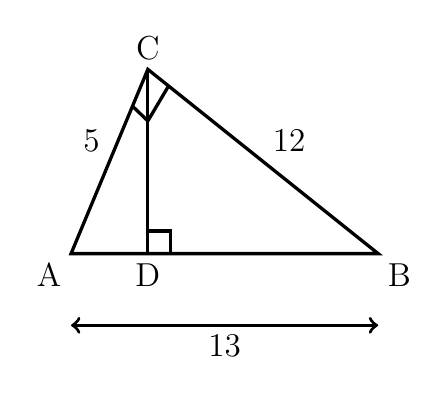
\begin{tikzpicture}[scale=1.3]

% Define vertices
\coordinate (A) at (0,0);
\coordinate (B) at (3,0);
\coordinate (D) at (0.75,0);
\coordinate (C) at (0.75,1.8);

% Draw triangle sides
\draw[very thick] (A) -- (C) -- (B) -- cycle;

% Draw altitude CD
\draw[very thick] (C) -- (D);

% Right angle mark at D
\draw[very thick] (D) ++(0.22,0) -- ++(0,0.22) -- ++(-0.22,0);

% Right angle square at C (angle ACB = 90°)
\coordinate (CA) at ($(C)!0.20!(A)$);  % Point along CA
\coordinate (CB) at ($(C)!0.09!(B)$);   % Point along CB
\coordinate (CC) at ($(C)!0.28!(D)$); % Corner of square
\draw[very thick] (CA) -- (CC) -- (CB);

% Arrow line below showing base length 13
\draw[very thick, <->] (0,-0.7) -- (3,-0.7);
\node[below] at (1.5,-0.7) {\large $13$};

% Vertex labels
\node[above] at (C) {\large C};
\node[below left] at (A) {\large A};
\node[below right] at (B) {\large B};
\node[below] at (D) {\large D};

% Side labels
\node[above left] at ($(A)!0.5!(C)$) {\large $5$};
\node[above right] at ($(C)!0.5!(B)$) {\large $12$};

\end{tikzpicture}
\end{document}